\documentclass[11pt]{amsart}
\usepackage{geometry}                % See geometry.pdf to learn the layout options. There are lots.
\geometry{letterpaper}                   % ... or a4paper or a5paper or ... 
%\geometry{landscape}                % Activate for for rotated page geometry
\usepackage[parfill]{parskip}    % Activate to begin paragraphs with an empty line rather than an indent
\usepackage{graphicx}
\usepackage{amssymb}
\usepackage{epstopdf}
\DeclareGraphicsRule{.tif}{png}{.png}{`convert #1 `dirname #1`/`basename #1 .tif`.png}
\usepackage{listings}
\usepackage{xcolor}
\usepackage{hyperref}
\usepackage{placeins}


\title{An Exploration of Atlanta Neighborhood Boundaries using KNN Classifiers}
\author{Katie Fullerton}
%\date{}                                           % Activate to display a given date or no date

\begin{document}
\lstset{    string=[s]{"}{"},
    stringstyle=\color{blue},
    comment=[l]{:},
    commentstyle=\color{black}
}
\maketitle
%------------------------------------------------------------------------------------------------
\section{Introduction}
%--------------------------------------------
\subsection{Background}
Atlanta is a major city in the south-eastern portion of the United States originally founded at the intersection of multiple railroad lines. As a city it has grown extensively in the last 50 years. Much of the planning efforts for that growth have been left to commercial developers, and consequently the city is somewhat a jumble of neighborhoods. Residents often complain that neighborhood boundaries are poorly-defined and have little connection with the actual usage patterns of the space. 
The city of Atlanta is divided into a number of Neighborhood Planning Units (NPUs). Each NPU is administered by a citizen and city employee council. These councils are empowered in various ways across the city, and have varying degrees of neighborhood buy-in. However, most NPUs do exert influence in the city zoning office, and thus can effect the type of development allowed within their borders. 
%--------------------------------------------
\subsection{Problem}
This system of NPUs was designed in the late 1970's. The past 50 years have seen dramatic shifts in population density, usage, and demographics in the Atlanta area. The purpose of this project is to compare the NPU boundaries designed in the 1970's to actual location usage patterns and determine if those boundaries still represent meaningful delineations.
This analysis would be of use to the city's planning board. If NPUs truly reflected the ways that citizens use their space, they would be more likely to get involved in the administration of those neighborhoods. Increased civic engagement has benefits both for the citizens and the city. This data might offer commercial value to developers looking to appeal to a specific consumer type, or to place new developments in areas of high likely usage.  
%------------------------------------------------------------------------------------------------
\section{Data}
%--------------------------------------------
\subsection{Data Sources}
In order to perform the analysis, we will need two separate data sets. The first required data set is the geospatial boundary data for each NPU, as designed in the 1970's. The second required data set must capture current usage patterns of the spaces in those geospatial regions. For the first dataset, we will access the City of Atlanta's GIS System via their website. The second dataset will be collected through the Foursquare API. It is assumed that Foursquare data represents real-time, up to date information about the way people live, work, and play in their neighborhoods.
\subsubsection{Geospatial Data}
The City of Atlanta offers a useful API explorer at \url{https://dcp-coaplangis.opendata.arcgis.com/datasets/npu/geoservice} . The resulting json file contains the information below. The fields of interest for this investigation are the NAME and geometry fields. 

\begin{lstlisting}
 { "attributes": {
            "OBJECTID": 260,
            "LOCALID": null,
            "NAME": "K",
            "GEOTYPE": "NPU",
            "FULLFIPS": null,
            "LEGALAREA": null,
            "ACRES": 1528.29,
            "SQMILES": 2.39,
            "OLDNAME": null,
            "NPU": null
         },
         "geometry": {
            "rings": [
               [
                  [
                     -84.4173772073577,
                     33.772197013770004
                  ],
\end{lstlisting}

Using this tool, we generated a request URL \url{https://gis.atlantaga.gov/dpcd/rest/services/OpenDataService/FeatureServer/4/query?where=1%3D1&outFields=NAME&outSR=4326&f=json} to create a simplified output object with only the fields of interest. 
\subsubsection{Location Usage Data}
In order to collect a sufficient amount of data for the large geographical area covered, we created a latitude and longitude search grid. This grid was set to contain 10 steps between the minimum and maximum latitude and longitude values present in the GIS data. The resulting search grid can be seen in Figure \ref{fig:gridmap}. For each coordinate in Figure \ref{fig:gridmap}, a url was generated to query the Foursquare API. An anonymized sample URL is: \url{https://api.foursquare.com/v2/venues/explore?client_id=XXXXXXXX&client_secret=XXXXXXX&ll=33.886869733912235,-84.28962468321286&v=20180604&limit=50&radius=4500}.
The results of each API call were compiled into a single large dataframe for cleaning.
\begin{figure}
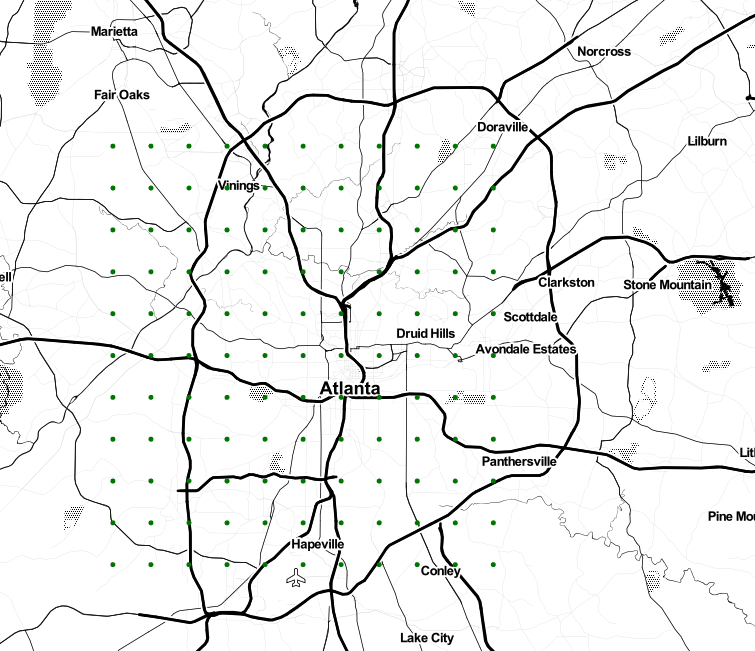
\includegraphics[width=\textwidth]{gridmap}
\caption{Latitude and Longitude Search Grid}
\label{fig:gridmap}
\end{figure}
\FloatBarrier
%--------------------------------------------
\subsection{Data Cleaning}
\subsubsection{Cleaning Geospatial Data}
After tailoring the API call to return only applicable data, the geospatial data set is structured with an array of coordinates representing the boundary in each row, as shown in Figure \ref{fig:gisresults}. In order to extract this data into a useful structure, the code below iterated through the GIS results and stored the latitude and longitude coordinates along with the name of the NPU in a separate dataframe. The resulting cleaned dataframe is demonstrated in Figure \ref{fig:cleanedgeodata}. 

\begin{figure}
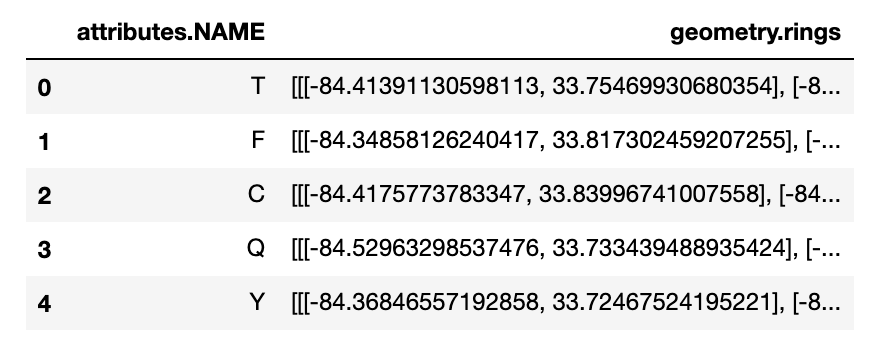
\includegraphics[width=0.5\textwidth]{gisresults}
\caption{Structured Data from The City of Atlanta's GIS System}
\label{fig:gisresults}
\end{figure}

\begin{lstlisting}[caption={Geospatial Data Cleaning Algorithm}]
gis_df = pd.DataFrame(columns=['NPU', 'Latitude','Longitude'])
for index, row in cleandata.iterrows():
    coord = row['geometry.rings'][0][:]
    name = row['attributes.NAME'][0][:]
    for ll in coord:
        lat = ll[1]
        long = ll[0]
        gis_df = gis_df.append({"NPU": name,"Latitude":lat,"Longitude": long}, ignore_index=True)
\end{lstlisting}

\begin{figure}
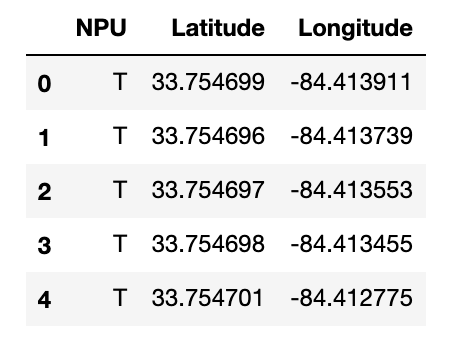
\includegraphics[width=0.3\textwidth]{cleanedgeodata}
\caption{Cleaned Geospatial Dataframe}
\label{fig:cleanedgeodata}
\end{figure}
\FloatBarrier
\subsubsection{Cleaning Location Usage Data}
Once retrieved, the location usage data contains significantly more data than needed for this analysis. The initial output format can be seen in Table \ref{tab:fsraw}

\begin{figure}[h]
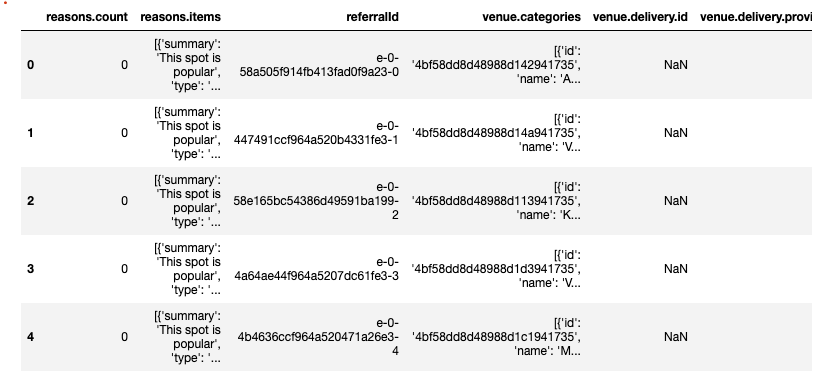
\includegraphics[width=0.8\textwidth]{Foursquare_API_output_table_raw}
\caption{Raw data output from Foursquare}
\label{tab:fsraw}
\end{figure}

The name, latitude, and longitude attributes could be directly extracted. The category field contained additional structure, so a function was written to extract the category string from that structure, as shown below. 
Initially, it appeared that the Foursquare data did include a neighborhood categorization. However, as the analysis continued, it became apparent that this field is either 'NaN' or left out of the data set entirely. While processing, a conditional clause was created, as seen below, to facilitate the compilation of the data.  In the final model, this data was determined to offer no additional value to the analysis. 

\lstset{language=Python}
\begin{lstlisting}[caption={Category Extraction Function}]
def get_category_type(row):
    try:
        categories_list = row['categories']
    except:
        categories_list = row['venue.categories']
        
    if len(categories_list) == 0:
        return None
    else:
        return categories_list[0]['name']
\end{lstlisting}

\begin{lstlisting}[caption={Neighborhood Data Screening Clause}]
 if 'venue.location.neighborhood' in list(dataframe.columns.values):
        data['neighborhood'] = dataframe['venue.location.neighborhood']
    else: 
        data['neighborhood'] = np.nan
        
\end{lstlisting}
\begin{figure}
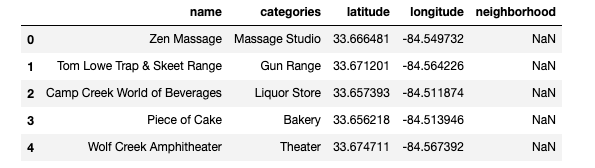
\includegraphics[width=0.8\textwidth]{Foursquare_API_output_table_cleaned}
\caption{Cleaned Location Dataframe}
\label{tab:fsclean}
\end{figure}

The search grid was constructed orthogonally, while the Foursquare interface assumes a circular search radius. Consequently, there are likely to be a number of locations that are captured in more than on API call. Duplicate data does not provide additional information for this analysis, and so duplicates were removed. The initial search resulted in 5901 total location listings, with only 2153 unique values. It was determined that this is a sufficient number for training and testing of a model. However, correcting the discrepancy between square and circular searches could increase the number of unique data points for future work. 
\FloatBarrier
%--------------------------------------------
\subsection{Exploratory Data Analysis}
\subsubsection{NPU Boundaries}
The NPU boundaries were described by a series of coordinates for each boundary. Figure \ref{fig:npuoutlines} shows each NPU boundary point. Note that the NPU's encompass primarily the western side of the city. Unfortunately, we do not have NPU data for the east side of the city due to cross-county policies that do not interact. Because of this skew, the search grid was tagged to the maximas and minimas of the NPU boundary coordinates. Future work could include data from additional counties to completely cover the metro Atlanta neighborhood. 
\begin{figure}[h]
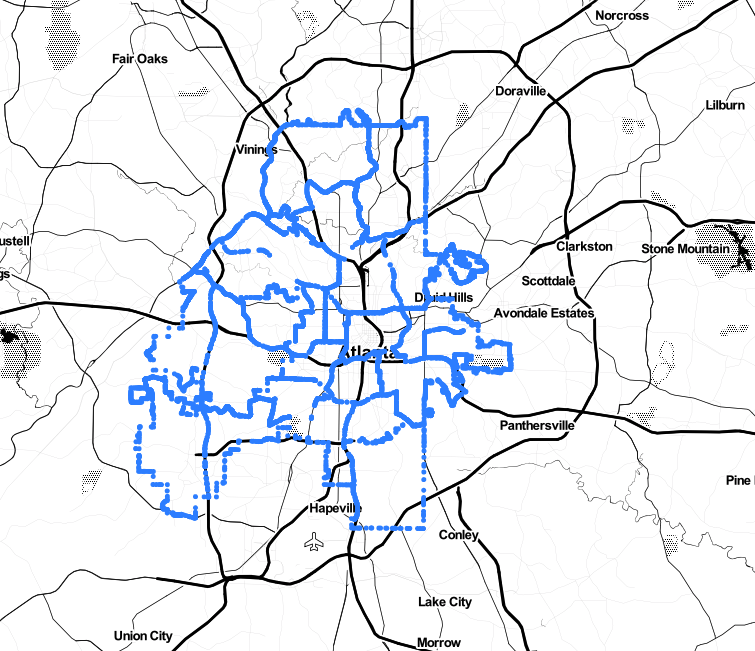
\includegraphics[width=\textwidth]{NPUoutlines.png}
\caption{NPU Boundaries in the City of Atlanta}
\label{fig:npuoutlines}
\end{figure}
\subsubsection{Foursquare Venue Data}
After performing the grid search and subsequent series of API calls, we can plot all the locations listed in the dataframe. Figure \ref{fig:venues} shows a blue point for each venue. We perform this visual analysis to verify that the venues correspond roughly to the search grid points. 
\begin{figure}[h]
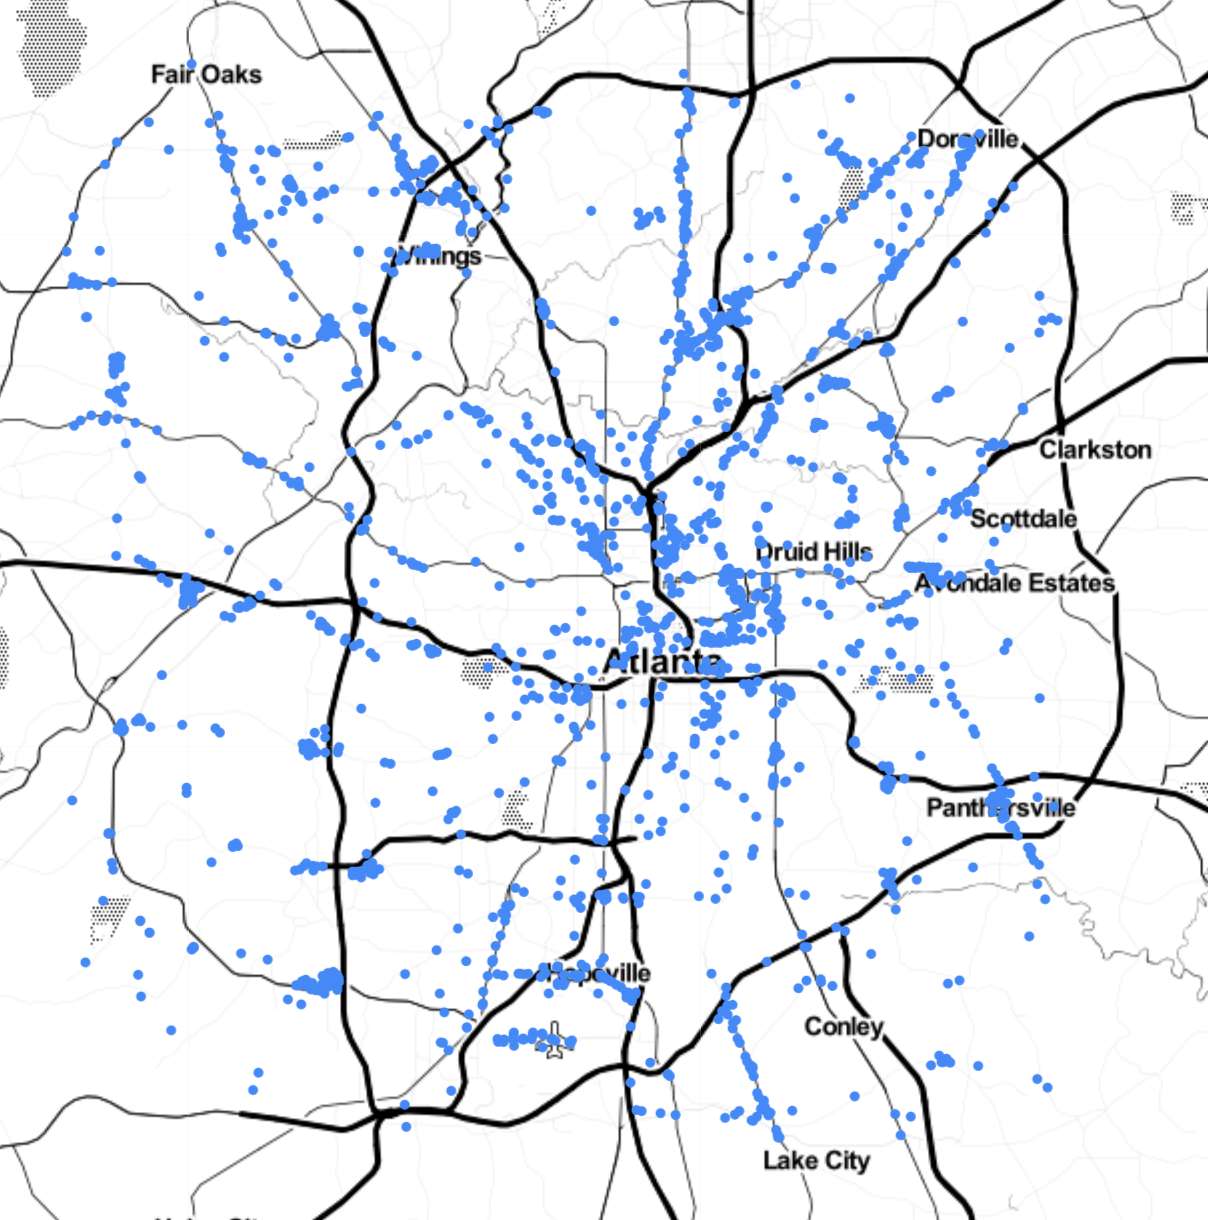
\includegraphics[width=\textwidth]{VenuesMap}
\caption{Results of Foursquare API call}
\label{fig:venues}
\end{figure}

Figure \ref{fig:catcounts} shows the count of venues by category from Foursquare. Clearly, there are a large number of categories with a single venue listed, which suggests that this category information will not provide additional information for this analysis. 
\begin{figure}
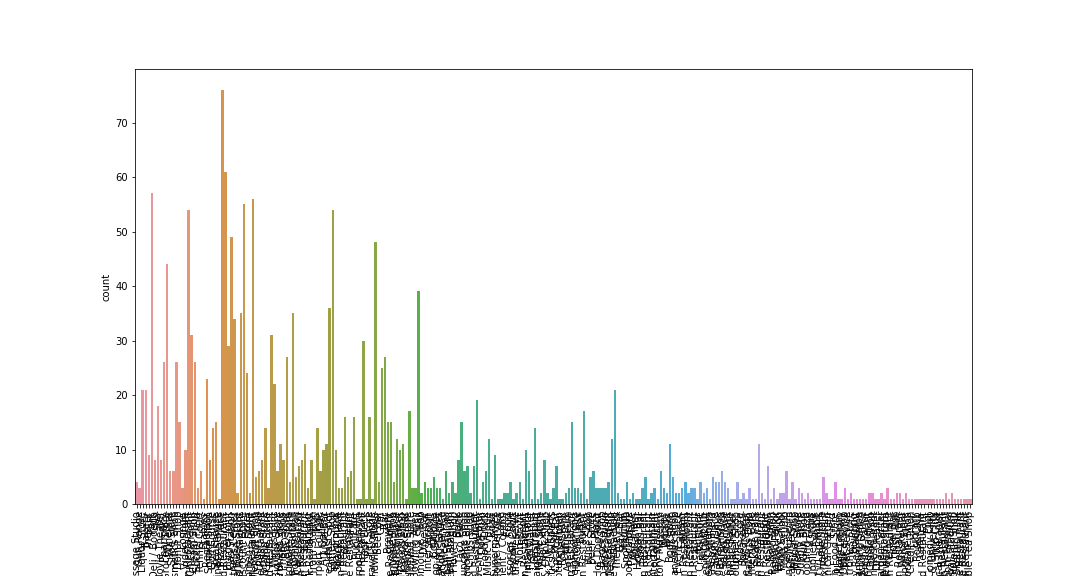
\includegraphics[width=\textwidth]{catcounts}
\caption{Count of Venues by Foursquare Category}
\label{fig:catcounts}
\end{figure}

\subsubsection{Intersection of Both Datasets}
After assigning each venue to an NPU, it is possible to plot the number of venues assigned to each NPU, as seen in Figure \ref{fig:npucounts}. This information will be used later to set the number of cross validation folds, since each fold must include at least one point from every category. Two of our NPU's contain less than 4 points, which will limit our number of cross validation folds to 3. If we wished to exclude these NPU's and their associated venues, we might be able to increase the accuracy of the model by introducing additional folds. 

\begin{figure}
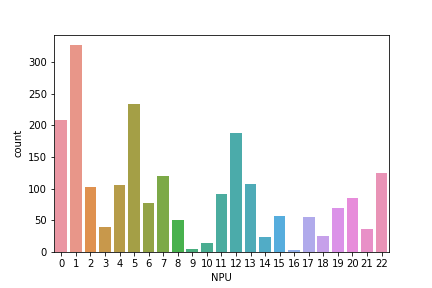
\includegraphics[width=0.5\textwidth]{NPUcounts}
\caption{Number of Venues in Each NPU}
\label{fig:npucounts}
\end{figure}
\FloatBarrier
%------------------------------------------------------------------------------------------------
\section{Methodology}
%--------------------------------------------
\subsection{NPU Assignment}
In order to assign each Foursquare location to an NPU, we created a simplified array with each NPU boundary coordinate and the corresponding NPU name. Then for each location retrieved from Foursquare, the Euclidean distance was calculated from the venue location to each boundary point. This vector of distances was searched for the minimum value, and the corresponding NPU name was stored for that venue. 
This method is a rough approximation- for instance, it does not consider any topographic or geographic conditions. However, given the time limits of this project, it was determined that this approximation was sufficient. Additional work could be done to refine this assignment method using GIS tools.
%--------------------------------------------
\subsection{KNN Classifier Construction}
We used the K Neighbors Classifier model available in sklearn. Our input matrix included the latitude and longitude of the Foursquare venues, and our classifier was the NPU assigned to each point. The data were split into test and training sets, with 80 \% for training and 20 \% for testing. 
%--------------------------------------------
\subsection{Cross Validation}
The primary tuning parameter for a KNN classifier is k. In order to select an appropriate k value for this analysis, we calculated the cross validation score for the KNeighborsClassifier with k values ranging from 1-10. The code for this evaluation can be seen below. The NPU with the smallest number of venues assigned had only 4 points, which forced us to use a 3 fold cross validation, since $n_{cross val} < n_{min num points}$. The resulting scores can be seen in Figure \ref{fig:kval}. 
This plot does not show a characteristic elbow that is often used in k-value selection. However, there are 2 points at which the slope significantly decreases: k = 2 and k = 4. Using k = 2 does not offer much useful information, so k = 4 was selected for the remainder of the analysis. 
\begin{figure}[h]
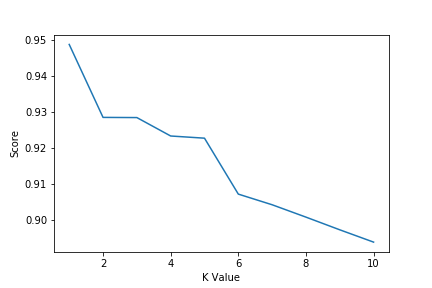
\includegraphics[width=0.7\textwidth]{kvalues}
\caption{Cross Validation Score for Various K Values}
\label{fig:kval}
\end{figure}

\begin{lstlisting}[caption={Cross Validation Testing}]
neighbors = list(range(1,11,1))
cv_scores = []
for k in neighbors:
    knn = KNeighborsClassifier(n_neighbors=k)
    scores = cross_val_score(knn, X_train, y_train, cv=3, scoring='accuracy')
    cv_scores.append(scores.mean())
\end{lstlisting}   

\FloatBarrier
%------------------------------------------------------------------------------------------------
\section{Results}
%--------------------------------------------
\subsection{Scoring}
Using the knn.score method available in the sklearn library. As can be seen in Figure \ref{fig:kval}, the score for the model is approximately 0.941, which indicates that the model does a fairly good job of classifying the test data. 
%--------------------------------------------
\subsection{Visual Analysis}
Since the goal of this analysis was to determine how realistic the old NPU boundaries are, we will use a visual analysis to see if the KNeighborsClassifier grouped venues in regions similar to the NPU system. Figure \ref{fig:preds} shows each of these test points. The color for each point indicates the accuracy of the model. If the initially assigned NPU matched the predicted NPU, the point was colored green. If not, the point was colored red. Clearly the green points outnumber the red points, which is in keeping with the score assigned above. 
The few red points likely lie along the NPU boundaries, where they might be assigned to one NPU but lie within a neighborhood that is irregularly shaped. 

\begin{figure}[h]
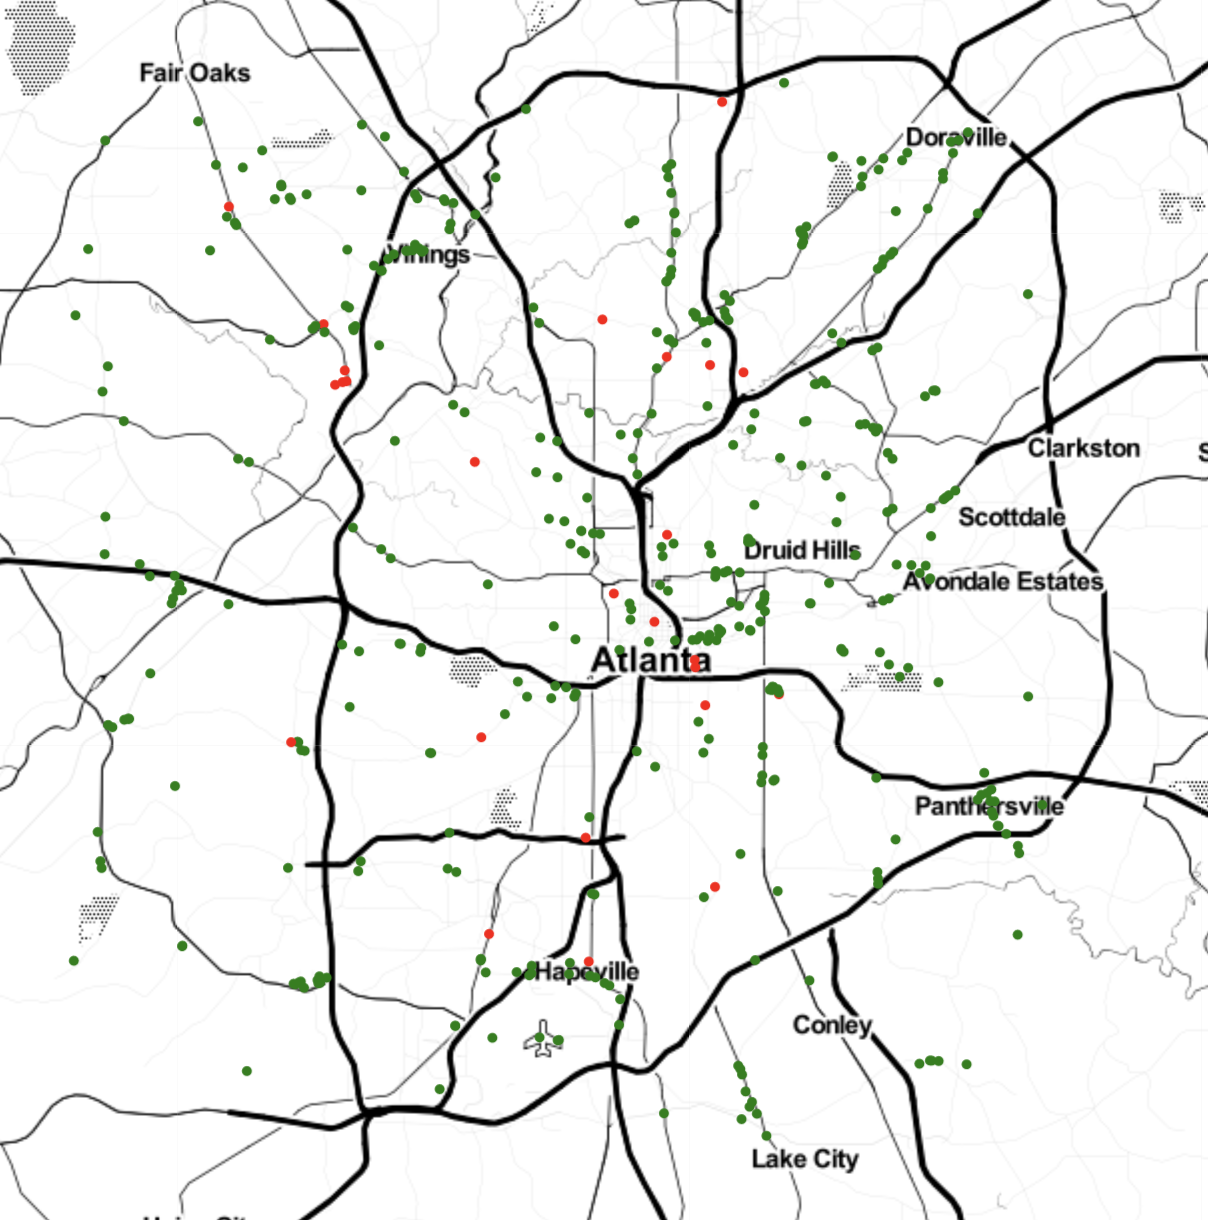
\includegraphics[width=\textwidth]{predictions}
\caption{Test Venues}
\label{fig:preds}
\end{figure}
\FloatBarrier
%------------------------------------------------------------------------------------------------
\section{Discussion}
Based on the score produced by sklearn, it seems that the KNN classifier does a decent job of predicting the neighborhood for a given venue. When viewed on a map, it becomes apparent that there is a systemic bias to the data. Misclassifications are overwhelmingly focused in the south-west portion of the city, while the north and east portion of the city are almost entirely correctly classified. 
This skew is likely due to two issues:
\begin{itemize}
\item Population density is higher in the north and east portions of the city, and lower in the southwest. This could result in a lower number of venues reported to Foursquare in that region, and thus an underlying bias in the dataset.
\item Due to lower population density, the NPU's in the southwest corner of the city are larger. This means that a point lies near the edge of an NPU may be classified in a different neighborhood by the nearest neighbors classifier. This error is a function of the way we classified venues into NPU's. We used an approximation to determine which boundary each venue was closest to in the classification, while the KNN algorithm considers irregular boundaries. Mitigation strategies are described in the next section.

\end{itemize}
%------------------------------------------------------------------------------------------------
\section{Conclusion}
Within the boundaries of the provided NPU geospatial data, it appears that the K Neighbors Classifier performs fairly well, and that the results of using it to predict a neighborhood assignment corresponds well with the NPU assignment described above. This would suggest that the NPU boundaries do still reflect actual use patterns. 
There are a number of assumptions that were used to simplify this analysis, including the method of assigning a venue to an NPU, and the method of assessing prediction accuracy visually. However, the correspondence between the assigned and predicted NPU does suggest that the NPU system is not as outdated as was originally assumed. This conclusion could be used to encourage citizens to participate in their NPU, as well as assure developers that the nature of the administrative boundaries is similar to the real life usage. 
\subsection{Future Work}
Throughout this report, a number of extensions have been suggested. They are summarized here. 
\begin{itemize}
\item Modifying the method of classifying venues into neighborhoods:
\begin{itemize}
\item Incorporating the Foursquare neighborhood classification: this was excluded due to the limited amount of data with information for that field. However, we could exclude those data points without a value and simply search for more venues that do have the data. 
\item  Using GIS data capabilities: With additional time and resources, the GIS data could be used to create more accurate determinations. However, that level of exploration was deemed beyond the scope of this work.
\end{itemize}
\item Search grid expansion: Our search grid was limited by the boundaries of the City of Atlanta. With further time, we could connect to the data systems for other local municipalities, and expand our search to cover the entire Atlanta area. 
\item Increasing the number of cross-validation folds used: the cross validation method was limited by the small number of venues in two of the NPU's. In additional analysis, we could exclude those two NPU's and perform a more rigorous cross validation. 
\end{itemize}


%------------------------------------------------------------------------------------------------
\end{document}  